\documentclass[review]{elsarticle}
% \usepackage[active, tightpage]{preview}

\usepackage{enumitem}
\usepackage{hyperref}
\usepackage{xcolor}
\hypersetup{
    colorlinks,
    linkcolor={red!50!black},
    citecolor={blue!50!black},
    urlcolor={blue!80!black},
    pdfborder={0 0 0}
}
\usepackage{multirow}
\usepackage{pgfplots}
\usepackage{float}
\usepackage{amssymb}
\usepackage{cleveref}
\usepackage[english]{babel}
\usepackage[utf8]{inputenc}
\usepackage[T1]{fontenc}
% \usepackage{changepage}
\usepackage{longtable}
\usepackage{tabularx}
\usepackage{pdfpages}
\usepackage{incgraph,tikz}
\usepackage[titles]{tocloft}
\setlength{\cftbeforesecskip}{-.5ex}
\renewcommand{\cftsecleader}{\cftdotfill{\cftdotsep}}

% \usepackage[showframe=true]{geometry}
%
\newcommand{\te}[1] {\texttt{\footnotesize#1}}
\newcommand{\h} {\hphantom ~ }
% \newcommand{\te}[1] {\mbox{\texttt{\footnotesize#1}}}
% \newcommand{\te}[1] {
% \begin{verbatim} #1 \end{verbatim}
% }
\pgfplotsset{compat=1.5}
\pgfplotsset
{
	width=0.5\textwidth,
	x tick label style={/pgf/number format/1000 sep=},
  enlarge x limits = 0.0,
  ymajorgrids=true,
	major tick style={draw=none},
  ymin = 0.0,
	every axis/.append style={
		every x tick label/.append style={font=\tiny},
    every y tick label/.append style={font=\tiny},
    every axis label/.append style={font=\small},
    height=37mm,
    width=37mm,
    title style={at={(0.5,0.90)}, font=\normalfont},
    xticklabel style={yshift=4pt}
	}
}

%% `Elsevier LaTeX' style
\bibliographystyle{elsarticle-num}
%
\makeatletter
\def\ps@pprintTitle{%
    \let\@oddhead\@empty
    \let\@evenhead\@empty
    \def\@oddfoot{}%
\let\@evenfoot\@oddfoot}
\makeatother
\begin{document}
%
\begin{frontmatter}
%
\title{LOSD: A Linked Open Social Dataset for Scientific Research
  (Supplementary document)}
%
\author[pwa]{Renato Fabbri\corref{corresponding}\fnref{kii-url}}
\ead{fabbri@usp.br}
%
\author[pwr]{Osvaldo Novais de Oliveira Junior\fnref{kio-url}}
\ead{chu@ifsc.usp.br}
%
\cortext[corresponding]{Corresponding author}
\address[pwa]{
Institute of Mathematical and Computer Sciences, University of São Paulo (ICMC/USP), São Carlos, Brazil
}
\address[pwr]{
São Carlos Institute of Physics, University of São Paulo (IFSC/USP), São Carlos, Brazil
}
%
\fntext[kii-url]{\textit{URL:} \url{https://icmc.usp.br/}}
\fntext[kio-url]{\textit{URL:} \url{http://www.ifsc.usp.br/}}
%
\begin{abstract}
This is a Supplementary document which provides ontological
diagrams and auxiliary tables for the LOSD dataset.
The main document of the article is in~\cite{losd}.
\end{abstract}
%
\end{frontmatter}
\newcommand{\foo}{\textheight}
\newcommand{\foobar}{\pdfpageheight}
% \pdfpageheight 8in
\tableofcontents
\clearpage
\section{General guidance}
% \paperheight = 200pt
In this document we provide diagrams
for the provenances in LOSD, namely
Facebook, Twitter, IRC, Email, Participa.BR, Cidade Democrática and AA.
Each provenance has two diagrams: one presents the relations
among classes (blue nodes) and data types (orange nodes),
the other presents metadata for the snapshot provenance.
Every class instance is related to the snapshot instance
by the triple \te{class\_uri po:snapshot snapshot\_uri}.
Such triples are omitted for simplicity.
Due to the large number of relations, the rendering of diagrams are
automatized and displays some overlaps of the nodes related to each class or datatype.
Even so, the images are useful for grasping what is available in current LOSD
and exploration assistance.
Edges in the diagrams have (see OWL official documentation or the article~\cite{losd}:
\begin{itemize}
    \item green color if representing an OWL existential
class restriction;
    \item inverted arrow tip if representing an OWL universal class
        restriction;
    \item full edges (non-dashed) if representing a functional property
        axiom.
\end{itemize}

Furthermore, this document ends with two sets of tables, one with
references for snapshot groups, such as Wikipedia or
contact links, 
the other with 
counts of
triples, participants, edges/interactions/relations and characters.


\section{Facebook data}
Each Facebook snapshot is yield by either a user, from which the
friends are in the friendship network, or a group, in which participants
can yield friendship and interaction networks and posts information with
text and some metadata.
Further information is found in the following diagrams, in the tables at
the end of this document or in the main document of this article~\cite{losd}.

% 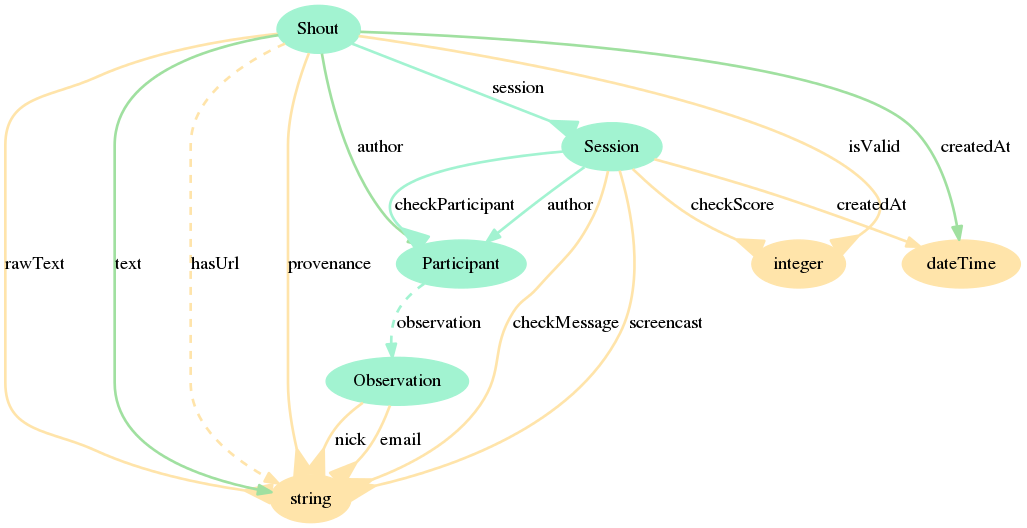
\includepdf{ontologies/aairc.ttl/draw.pdf}
\incgraph[
  overlay={\node[red,below right] at (page.north west) {\Huge Facebook};}
    paper=graphics
][scale=.6]{ontologies/facebook-legacy-Auricultura10042013Friendship.ttl/draw.png}

\textheight = 2in
\pdfpageheight 5in
\incgraph[
  overlay={\node[red,below right] at (page.north west) {\Huge Facebook};}
    paper=graphics
][scale=.5]{ontologies/facebook-legacy-Auricultura10042013Meta.ttl/draw.png}

\section{Twitter data}
Each Twitter snapshot is yield by a hashtag.
Retweets (\te{po:retweetOf} are usually considered the interactions between users.
The database present also \te{po:replyTo} and \te{po:userMention}
which may be useful in understanding the networking and provides additional networks.
Further information is found in the following diagrams, in the tables at
the end of this document or in the main document of this article~\cite{losd}.

\incgraph[
  overlay={\node[red,below right] at (page.north west) {\Huge
  Twitter };}
    paper=graphics
][scale=.5]{ontologies/twitter-legacy-arenaNETmundialTweet00000.ttl/draw.png}

\incgraph[
  overlay={\node[red,below right] at (page.north west) {\Huge Twitter};}
    paper=graphics
][scale=.7]{ontologies/twitter-legacy-arenaNETmundialMeta.ttl/draw.png}

\section{IRC data}
Each IRC snapshot is yield by an IRC channel.
IRC messages are either 1) server messages (e.g. join and exit)
marked with \te{po:systemMessage true} and having an \te{po:impliedUser user\_uri},
or 2) user messages, which yield interactions through \te{po:directedTo} and \te{po:mentions} properties.
Text messages without the user names are provided through the \te{po:cleanText} property.
Further information is found in the following diagrams, in the tables at
the end of this document or in the main document of this article~\cite{losd}.
\incgraph[
  overlay={\node[red,below right] at (page.north west) {\Huge IRC};}
    paper=graphics
][scale=.7]{ontologies/irc-legacy-hackerspace-cpsLog00000.ttl/draw.png}
\incgraph[
  overlay={\node[red,below right] at (page.north west) {\Huge IRC};}
    paper=graphics
][scale=.6]{ontologies/irc-legacy-hackerspace-cpsMeta.ttl/draw.png}

\section{Email data}
Each email snapshot is yield by an Email list.
Interactions are entailed by \te{po:replyTo} relations
although \te{po:to} and \te{po:cc} may also be considered.
The email body is given by \te{po:text} relations while
\te{po:cleanText} links to text with lines removed where they are
obviously from previous messages or computer code.
Further information is found in the following diagrams, in the tables at
the end of this document or in the main document of this article~\cite{losd}.
\incgraph[
  overlay={\node[red,below right] at (page.north west) {\Huge Email};}
    paper=graphics
][scale=.4]{ontologies/email-legacy-linux.audio.devel1-20000Email00000.ttl/draw.png}
\textheight = 3in
\pdfpageheight 6in
\incgraph[
  overlay={\node[red,below right] at (page.north west) {\Huge Email};}
    paper=graphics
][scale=.5]{ontologies/email-legacy-linux.audio.devel1-20000Meta.ttl/draw.png}

\section{Participa.BR data}
The Participa.BR snapshot is yield by a data dump donated by the system
administrators of the federal portal of social participation Participa.BR.
Articles can have parent articles (\te{po:parent}), can be a step of a
collection of articles (\te{po:stepOf}) and can be a mediation of other
articles (\te{po:mediationOf}).
Interactions are entailed by comments which are \te{po:replyTo} other
comments or which are made directly to an article.
This snapshot also holds friendship structures.
The language used is mainly Brazilian Portuguese, but English and
Spanish are also incident.
Due to the higher complexity of the diagram, an additional figure,
obtained through another layout algorithm, is given.
Further information is found in the following diagrams, in the tables at 
the end of this document or in the main document of this article~\cite{losd}.
\incgraph[
  overlay={\node[red,below right] at (page.north west) {\Huge
  Participa.BR};}
    paper=graphics
][scale=.5]{ontologies/participabr.ttl/draw.png}
\incgraph[
  overlay={\node[red,below right] at (page.north west) {\Huge
  Participa.BR};}
    paper=graphics
][scale=.7]{ontologies/participabr.ttl/draw_circo.png}
\incgraph[
  overlay={\node[red,below right] at (page.north west) {\Huge
  Participa.BR};}
    paper=graphics
][scale=.7]{ontologies/participabrMeta.ttl/draw.png}

\section{Cidade Democrática data}
The Cidade Democrática snapshot is yield by a data dump donated by the system
administrators of the civil society social participation portal Cidade
Democrática.
This snapshot holds a complex structure of both
Topics/Inspirations/Observatories/Supports/Competitions/Prizes
and of State/City/Neighborhood/Place.
The language used is mainly Brazilian Portuguese.
Due to the higher complexity of the diagram, an additional figure,
obtained through another layout algorithm, is given.
Further information is found in the following diagrams, in the tables at
the end of this document or in the main document of this article~\cite{losd}.
\incgraph[
  overlay={\node[red,below right] at (page.north west) {\Huge Cidade
  Democrática};}
    paper=graphics
][scale=.4]{ontologies/cidadedemocratica00000.ttl/draw.png}
\textheight = 2in
\pdfpageheight 5in
\incgraph[
  overlay={\node[red,below right] at (page.north west) {\Huge Cidade
  Democrática};}
    paper=graphics
][scale=.4]{ontologies/cidadedemocratica00000.ttl/draw_circo.png}

\incgraph[
  overlay={\node[red,below right] at (page.north west) {\Huge Cidade
  Democrática};}
    paper=graphics
][scale=.7]{ontologies/cidadedemocraticaMeta.ttl/draw.png}

\section{AA data}
The AA (Algorithmic Autoregulation) snapshots are yield by a data dump donated by the system
administrators and by a mined IRC log.
The system aims at simplicity and most of the data consists of
shouts with \te{po:text} and \te{po:author}.
Further information is found in the following diagrams, in the tables at
the end of this document or in the main document of this article~\cite{losd}.
\incgraph[
  overlay={\node[red,below right] at (page.north west) {\Huge AA};}
    paper=graphics
][scale=.6]{ontologies/aairc.ttl/draw.png}
\textheight = 7in
\pdfpageheight \foobar
\incgraph[
  overlay={\node[red,below right] at (page.north west) {\Huge AA};}
    paper=graphics
][scale=.7]{ontologies/aaircMeta.ttl/draw.png}

\section{Snapshot references}
\label{sreferences}
\pdfpageheight 10in
\begin{table*}[h!]
\begin{center}\scriptsize
\caption{All the Facebook snapshots are either the result of individuals who downloaded
their data (and donated to the first author) or data downloaded from groups.
In the first case, it is senseless to present references. In the second
case, we present the group name and a link to a post in the group where
data and figures were delivered back to the group.}
\begin{tabular}{| l | p{9.9cm} |}\hline
\textbf{group name} & \textbf{url(s)} \\\hline
Adorno Nao Eh Enfeite & \url{https://www.facebook.com/groups/265217103529531/permalink/525654127485826/} \\\hline
Ativistas Da Inclusao Digital & \url{https://www.facebook.com/groups/423602557691243/permalink/525201037531394/} \\\hline
Ciencias Com Fronteiras & \url{https://www.facebook.com/groups/contraaexclusao/permalink/269103356558439/} \\\hline
Computer Art & \url{https://www.facebook.com/groups/computerart/permalink/259389137529870/} \\\hline
Coolmeia &  \url{https://www.facebook.com/groups/coolmeia/permalink/380091142098291/} , \url{https://www.facebook.com/groups/coolmeia/permalink/489757754464962/} \\\hline
Democracia Direta Ja & \url{https://www.facebook.com/groups/ddjbrasil/permalink/347023325397298/} \\\hline
Democracia Pura & \url{https://www.facebook.com/groups/democraciapura/permalink/310907215704321/} \\\hline
Economia & \url{https://www.facebook.com/groups/economa1/permalink/586007714743535/} \\\hline
Economia Criativa Digital & \url{https://www.facebook.com/groups/economiacriativadigital/permalink/438313682916103/} \\\hline
Educacoes E Aprendizagens XXI & \url{https://www.facebook.com/groups/geaxxi/permalink/433229973421182/} \\\hline
Latesfip & \url{https://www.facebook.com/groups/183557128478424/permalink/266610616839741/} \\\hline
Living Bridges Planet & \url{https://www.facebook.com/groups/livingbridgesplanet/permalink/352950408144951/} \\\hline
Mobilizacoes Culturais Interior SP & \url{https://www.facebook.com/groups/131639147005593/permalink/144204529082388/} \\\hline
Partido Pirata & \url{https://www.facebook.com/groups/partidopiratabrasil/permalink/10151409024509317/} \\\hline
Politicas Culturas Brasileiras & \url{https://www.facebook.com/groups/pcult/permalink/519626544747423/} \\\hline
Praca Popular & \url{https://www.facebook.com/groups/215924991863921/permalink/319279541528465/} \\\hline
Rede Tranzmidias & \url{https://www.facebook.com/groups/318333384951196/permalink/346658712118663/} \\\hline
Silicon Valley Global Network & \url{https://www.facebook.com/groups/109971182359978/permalink/589326757757749/} \\\hline
Solidarity Economy & \url{https://www.facebook.com/groups/9149038282/permalink/10151461945623283/} \\\hline
Study Group SNA & \url{https://www.facebook.com/groups/140630009439814/permalink/151470598355755/} \\\hline
Tecnoxamanismo &  \url{https://www.facebook.com/groups/505090906188661/permalink/733144993383250/} , \url{https://www.facebook.com/groups/505090906188661/permalink/733157380048678/} \\\hline
\end{tabular}\end{center}
\end{table*}




\begin{table*}[h!]\scriptsize
\begin{center}
\caption{Different Twitter snapshots are yield by different hashtags.
  This table presents each snapshot with the respective hashtag and a
reference to the subject.}\label{tab:provenance}
\begin{tabular}{| l || p{4cm} | p{4cm} | }\hline
    \textbf{snapshot hashtag} & \textbf{observation} & \textbf{reference} \\\hline\hline
    \#arenaNETmundial & a Brazilian discussion hub about free culture, democracy and the internet & \url{http://www.participa.br/netmundial} \\\hline
    \#art & tweets with the generic hashtag \#art & \url{https://en.wikipedia.org/wiki/Art} \\\hline
    \#ChennaiFloods & heavy rainfall generated by the annual northeast monsoon in November–December 2015 & \url{https://en.wikipedia.org/wiki/2015_South_Indian_floods} \\\hline
    \#dilma & the 36th President of Brazil & \url{https://en.wikipedia.org/wiki/Dilma_Rousseff} \\\hline
    \#ForaDilma & 2015-16 anti-government protests in Brazil & \url{https://en.wikipedia.org/wiki/2015-16_protests_in_Brazil} \\\hline
    \#ForaCunha & 2015-16 anti-corruption protests in Brazil & \url{https://en.wikipedia.org/wiki/2015-16_protests_in_Brazil} \\\hline
    \#fuck & tweets with the generic hashtag \#fuck & \url{https://en.wikipedia.org/wiki/Fuck} \\\hline
    \#game & tweets with the generic hashtag \#game & \url{https://en.wikipedia.org/wiki/Game} \\\hline
    \#god & tweets with the generic hashtag \#god & \url{https://en.wikipedia.org/wiki/God} \\\hline
    \#MAMA2015 & the grand 2015 Mnet Asian Music Awards & \url{https://en.wikipedia.org/wiki/2015_Mnet_Asian_Music_Awards} \\\hline
    \#music & tweets with the generic hashtag \#music & \url{https://en.wikipedia.org/wiki/Music} \\\hline
    \#obama & the 44th President of the United States & \url{https://en.wikipedia.org/wiki/Barack_Obama} \\\hline
    \#python & the Python programming language & \url{https://en.wikipedia.org/wiki/Python_(programming_language)} \\\hline
    \#QuartaSemRacismoClubeSDV & an anti-racism netweaving & \url{https://twitter.com/hashtag/quartasemracismoclubesdv} \\\hline
    \#science & tweets with the generic hashtag \#science & \url{https://en.wikipedia.org/wiki/Science} \\\hline
    \#SnapDetremura & reference for Snapchat about a celebrated person & \url{https://twitter.com/detremura} \\\hline
\end{tabular}\end{center}
\end{table*}                    


\begin{table*}[h!]\scriptsize
\begin{center}
\caption{Different IRC snapshots are yield by different IRC channels.
  This table presents each snapshot with the respective channel and a
reference to the subject.}\label{tab:provenance}
\begin{tabular}{| l || p{4cm} | p{4cm} | }\hline
    \textbf{snapshot channel} & \textbf{observation} & \textbf{reference} \\\hline\hline
    \#foradoeixo & a Brazilian network of culture related collectives & \url{https://pt.wikipedia.org/wiki/Fora_do_Eixo} \\\hline
    \#hackerspace-cps & a hackerspace in Campinas, Brazil & \url{https://lhc.net.br/wiki/P%C3%A1gina_principal} \\\hline
    \#hackerspaces-br & Brazilian hackerspaces channel & \url{https://garoa.net.br/wiki/Hackerspaces_Brasileiros} \\\hline
    \#labmacambira & Brazilian channel for the labMacambira collective & \url{http://labmacambira.sourceforge.net/} \\\hline
\end{tabular}\end{center}
\end{table*}                    

\begin{table*}[h!]\scriptsize
\begin{center}
\caption{Different Email snapshots are yield by different email lists.
  This table presents each snapshot with the respective list and a
reference to the subject.}\label{tab:provenance}
\begin{tabular}{| p{4cm} || p{4cm} | p{4cm} | }\hline
    \textbf{Gmane ID} & \textbf{observation} & \textbf{reference} \\\hline\hline
    gmane.linux.audio.users & the Linux Audio Users & \url{http://linuxaudio.org} \\\hline
    gmane.politics.organizations.me-tareciclagem & a network about technology and social transformation  & \url{https://metareciclagem.github.io} \\\hline
    gmane.linux.audio.devel & the Linux Audio Developers & \url{http://lists.linuxaudio.org/listinfo/linux-audio-dev} \\\hline
    gmane.comp.gcc.libstdc++.devel & the C++ standard library & \url{https://gcc.gnu.org/libstdc++/} \\\hline
\end{tabular}\end{center}
\end{table*}                    
 
\begin{table*}[h!]\scriptsize
\begin{center}
\caption{References for the snapshots of
Participa.BR, Cidade Democrática and AA.}\label{tab:provenance}
\begin{tabular}{| l || p{4cm} | p{3cm} | }\hline
    \textbf{social protocol} & \textbf{observations} & \textbf{reference} \\\hline\hline
    Participa.BR & a Brazilian federal portal of social participation & \url{http://www.participa.br/} \\\hline
    Cidade Demorática & a Brazilian civil society portal of social participation & \url{http://www.cidadedemocratica.org.br/} \\\hline
    AA & the Algorithmic Autoregulation software development methodology & \cite{aarticle} \\\hline
\end{tabular}\end{center}
\end{table*}                    


\clearpage
\section{Trivial counts in each snapshot}
\begin{center}
\scriptsize\begin{longtable}{| l | c | c | c | c |}
\caption{Number of triples (ntriples), number of relations/interactions/edges (nedges), number of participants (nparticipants) and number of characters (nchars) in each LOSD snapshot.}
\\
\hline
\textbf{snapshot id} & \textbf{ntriples}  & \textbf{nedges}  & \textbf{nparticipants}  & \textbf{nchars} \\\hline\hline
\endfirsthead
\multicolumn{5}{c}{\tablename\ \thetable\ -- \textit{Continued from previous page}} \\\hline
\textbf{snapshot id} & \textbf{ntriples}  & \textbf{nedges}  & \textbf{nparticipants}  & \textbf{nchars} \\\hline\hline\endhead
\hline \multicolumn{5}{r}{\textit{Continued on next page}} \\
\endfoot\hline\endlastfoot

aa-irc-legacy-foradoeixo.log & 22  & 0  & 1  & 0 \\\hline
aa-irc-legacy-hackerspace-cps.log & 36  & 0  & 2  & 0 \\\hline
aa-irc-legacy-hackerspaces-br.log & 64  & 0  & 5  & 0 \\\hline
aa-irc-legacy-labmacambira\_lalenia.txt & 53067  & 0  & 117  & 0 \\\hline
aa-mongo-legacy & 22773  & 0  & 37  & 0 \\\hline
aa-mysql-legacy & 790796  & 0  & 157  & 0 \\\hline
cidadedemocratica-legacy & 1548412  & 0  & 23079  & 0 \\\hline
facebook-legacy-AdornoNaoEhEnfeite29032013 & 8841  & 1292  & 293  & 26113 \\\hline
facebook-legacy-AntonioAnzoategui18022013 & 1852  & 328  & 52  & 0 \\\hline
facebook-legacy-AtivistasDaInclusaoDigital09032013 & 25642  & 5592  & 306  & 0 \\\hline
facebook-legacy-Auricultura10042013 & 19905  & 3898  & 412  & 14015 \\\hline
facebook-legacy-BrunoMialich31012013 & 40970  & 9320  & 502  & 0 \\\hline
facebook-legacy-CalebLuporini13042013 & 106138  & 24653  & 1050  & 0 \\\hline
facebook-legacy-CalebLuporini19022013 & 104922  & 24391  & 1026  & 0 \\\hline
facebook-legacy-CienciasComFronteiras29032013 & 110734  & 23302  & 2921  & 0 \\\hline
facebook-legacy-ComputerArt10032013 & 260050  & 62819  & 1342  & 0 \\\hline
facebook-legacy-Coolmeia06032013 & 76063  & 16534  & 1202  & 0 \\\hline
facebook-legacy-DanielPenalva18022013 & 3695  & 682  & 113  & 0 \\\hline
facebook-legacy-DemocraciaDiretaJa14032013 & 259061  & 59323  & 3053  & 54443 \\\hline
facebook-legacy-DemocraciaDiretaJa14072013 & 4162  & 310  & 214  & 58035 \\\hline
facebook-legacy-DemocraciaPura06042013 & 32627  & 6730  & 627  & 65062 \\\hline
facebook-legacy-Economia14042013 & 239190  & 54001  & 3587  & 52664 \\\hline
facebook-legacy-EconomiaCriativaDigital03032013 & 185905  & 43128  & 1684  & 0 \\\hline
facebook-legacy-EducacoesEAprendizagensXXI02032013 & 106918  & 24802  & 1285  & 0 \\\hline
facebook-legacy-GabrielaThume19022013 & 18757  & 4108  & 307  & 0 \\\hline
facebook-legacy-GrahamForrest28012013 & 1546  & 185  & 90  & 0 \\\hline
facebook-legacy-LailaManuelle17012013 & 201247  & 48572  & 969  & 0 \\\hline
facebook-legacy-LarissaAnzoategui20022013 & 25000  & 5191  & 580  & 0 \\\hline
facebook-legacy-Latesfip08032014 & 11554  & 2009  & 306  & 0 \\\hline
facebook-legacy-LivingBridgesPlanet29032013 & 150032  & 32494  & 3077  & 52808 \\\hline
facebook-legacy-LuisCirne07032013 & 16795  & 3390  & 437  & 0 \\\hline
facebook-legacy-MariliaMelloPisani10042013 & 84946  & 19040  & 1230  & 0 \\\hline
facebook-legacy-Mirtes16052013 & 39591  & 9075  & 445  & 0 \\\hline
facebook-legacy-MobilizacoesCulturaisInteriorSP13032013 & 26518  & 6096  & 298  & 0 \\\hline
facebook-legacy-PartidoPirata23032013 & 45883  & 8537  & 1943  & 36313 \\\hline
facebook-legacy-PedroPauloRocha10032013 & 216064  & 50591  & 1932  & 0 \\\hline
facebook-legacy-PeterForrest28012013 & 8332  & 1829  & 120  & 0 \\\hline
facebook-legacy-PoliticasCulturasBrasileiras08032013 & 178689  & 41690  & 1278  & 69756 \\\hline
facebook-legacy-PracaPopular16032013 & 4577  & 932  & 65  & 4249 \\\hline
facebook-legacy-RafaelReinehr09042013 & 174599  & 39586  & 2297  & 0 \\\hline
facebook-legacy-RamiroGiroldo20022013 & 10104  & 2020  & 264  & 0 \\\hline
facebook-legacy-RedeTranzmidias02032013 & 25497  & 4940  & 391  & 54907 \\\hline
facebook-legacy-RenatoFabbri02032013 & 93310  & 21579  & 974  & 0 \\\hline
facebook-legacy-RenatoFabbri03032013 & 93866  & 21711  & 978  & 0 \\\hline
facebook-legacy-RenatoFabbri11072013 & 114728  & 26440  & 1256  & 0 \\\hline
facebook-legacy-RenatoFabbri18042013 & 104332  & 24072  & 1124  & 0 \\\hline
facebook-legacy-RenatoFabbri20012013 & 86592  & 20085  & 868  & 0 \\\hline
facebook-legacy-RenatoFabbri29112012 & 82269  & 19083  & 823  & 0 \\\hline
facebook-legacy-RicardoFabbri18022013 & 11548  & 2327  & 344  & 0 \\\hline
facebook-legacy-RitaWu08042013 & 84071  & 18935  & 1165  & 0 \\\hline
facebook-legacy-RonaldCosta12062013 & 31514  & 6557  & 730  & 0 \\\hline
facebook-legacy-SiliconValleyGlobalNetwork27042013 & 77552  & 15740  & 2130  & 50251 \\\hline
facebook-legacy-SolidarityEconomy12042013 & 14614  & 2404  & 525  & 67774 \\\hline
facebook-legacy-StudyGroupSNA05042013 & 5856  & 480  & 448  & 25474 \\\hline
facebook-legacy-THackDay26032013 & 1844  & 420  & 41  & 0 \\\hline
facebook-legacy-Tecnoxamanismo08032014 & 11106  & 2069  & 318  & 0 \\\hline
facebook-legacy-Tecnoxamanismo15032014 & 14589  & 2702  & 450  & 0 \\\hline
facebook-legacy-ThaisTeixeira19022013 & 26600  & 6088  & 296  & 0 \\\hline
facebook-legacy-VilsonVieira18022013 & 19864  & 4334  & 336  & 0 \\\hline
facebook-legacy-ViniciusSampaio18022013 & 90691  & 21360  & 725  & 0 \\\hline
facebook-legacy-avlab\_BarthorLaZule22022014 & 16005  & 3513  & 279  & 0 \\\hline
facebook-legacy-avlab\_CalebLuporini25022014 & 125577  & 29268  & 1215  & 0 \\\hline
facebook-legacy-avlab\_CamilaBatista23022014 & 21138  & 4476  & 462  & 0 \\\hline
facebook-legacy-avlab\_CarlosDiego25022014 & 171744  & 39401  & 2020  & 0 \\\hline
facebook-legacy-avlab\_CristinaMekitarian23022014 & 24647  & 5572  & 337  & 0 \\\hline
facebook-legacy-avlab\_DanielGonzales23022014 & 196406  & 45318  & 2162  & 0 \\\hline
facebook-legacy-avlab\_FelipeBrait23022014 & 1228605  & 299082  & 4611  & 0 \\\hline
facebook-legacy-avlab\_FelipeVillela22022014 & 2475  & 477  & 81  & 0 \\\hline
facebook-legacy-avlab\_JoaoMeirelles25022014 & 52371  & 11649  & 825  & 0 \\\hline
facebook-legacy-avlab\_JoaoMekitarian23022014 & 88765  & 20821  & 783  & 0 \\\hline
facebook-legacy-avlab\_JulianaSouza23022014 & 129757  & 29942  & 1427  & 0 \\\hline
facebook-legacy-avlab\_KarinaGomes22022014 & 9073  & 1906  & 207  & 0 \\\hline
facebook-legacy-avlab\_LucasOliveira26022014 & 62871  & 14764  & 545  & 0 \\\hline
facebook-legacy-avlab\_MarcelaLucatelli25022014 & 138733  & 31647  & 1735  & 0 \\\hline
facebook-legacy-avlab\_MariliaPisani25022014 & 114765  & 25830  & 1635  & 0 \\\hline
facebook-legacy-avlab\_NatachaRena22022014 & 642769  & 154758  & 3391  & 0 \\\hline
facebook-legacy-avlab\_OrlandoCoelho22022014 & 5149  & 848  & 251  & 0 \\\hline
facebook-legacy-avlab\_PalomaKliss25022014 & 493774  & 119520  & 2242  & 0 \\\hline
facebook-legacy-avlab\_PedroRocha25022014 & 346883  & 81910  & 2749  & 0 \\\hline
facebook-legacy-avlab\_RenatoFabbri22022014 & 124703  & 28780  & 1369  & 0 \\\hline
facebook-legacy-avlab\_SarahLuporini25022014 & 505853  & 121502  & 2835  & 0 \\\hline
facebook-legacy-avlab\_SatoBrasil25022014 & 1519394  & 371249  & 4914  & 0 \\\hline
facebook-legacy-ego\_MarceloSaldanha19112014 & 130556  & 29440  & 1828  & 0 \\\hline
facebook-legacy-ego\_MariliaPisani06052014 & 122231  & 27581  & 1701  & 0 \\\hline
facebook-legacy-ego\_MassimoCanevacci19062013 & 273328  & 59995  & 4764  & 0 \\\hline
facebook-legacy-ego\_RenatoFabbri06022014 & 123993  & 28606  & 1367  & 0 \\\hline
facebook-legacy-ego\_RenatoFabbri19112014 & 153410  & 35514  & 1622  & 0 \\\hline
facebook-legacy-ego\_VJPixel23052014 & 231608  & 54752  & 1800  & 0 \\\hline
facebook-legacy-posavlab\_AnaCelia18032014 & 53939  & 12167  & 753  & 0 \\\hline
facebook-legacy-posavlab\_ElenaGarnelo04032014 & 93472  & 21723  & 940  & 0 \\\hline
facebook-legacy-posavlab\_FabiBorges08032014 & 159584  & 36592  & 1888  & 0 \\\hline
facebook-legacy-posavlab\_GeorgeSanders08032014 & 108071  & 24706  & 1321  & 0 \\\hline
facebook-legacy-posavlab\_GrazielleMachado18032014 & 24264  & 5254  & 464  & 0 \\\hline
facebook-legacy-posavlab\_RenatoFabbri19032014 & 129360  & 29890  & 1400  & 0 \\\hline
facebook-legacy-posavlab\_RicardoPoppi18032014 & 76104  & 17234  & 1024  & 0 \\\hline
gmane-legacy-.comp.gcc.libstdc++.devel1-20000 & 364045  & 14786  & 1036  & 30126252 \\\hline
gmane-legacy-.linux.audio.devel1-20000 & 418957  & 17076  & 1232  & 26969596 \\\hline
gmane-legacy-.linux.audio.users1-20000 & 390944  & 16362  & 1147  & 25065928 \\\hline
gmane-legacy-.politics.organizations.metareciclagem1-20000 & 378641  & 15230  & 477  & 54260954 \\\hline
irc-legacy-foradoeixo & 859401  & 4308  & 3318  & 3023060 \\\hline
irc-legacy-hackerspace-cps & 286886  & 1860  & 607  & 454655 \\\hline
irc-legacy-hackerspaces-br & 1347458  & 210  & 347  & 8029920 \\\hline
irc-legacy-labmacambira & 1964597  & 58525  & 1561  & 6535187 \\\hline
participabr-legacy & 198157  & 0  & 3825  & 0 \\\hline
twitter-legacy-ChennaiFloods & 7255622  & 86935  & 46493  & 23237802 \\\hline
twitter-legacy-ForaCunha & 95613  & 1406  & 2747  & 372131 \\\hline
twitter-legacy-ForaDilma & 28554  & 534  & 659  & 113810 \\\hline
twitter-legacy-MAMA2015 & 21736361  & 411971  & 33080  & 75358785 \\\hline
twitter-legacy-QuartaSemRacismoClubeSDV & 395019  & 4023  & 5785  & 1635867 \\\hline
twitter-legacy-SnapDetremura & 28896  & 405  & 621  & 124448 \\\hline
twitter-legacy-arenaNETmundial & 414868  & 13291  & 5898  & 2825121 \\\hline
twitter-legacy-art & 2980883  & 26501  & 30486  & 9539413 \\\hline
twitter-legacy-dilma & 83663  & 1563  & 2274  & 332005 \\\hline
twitter-legacy-fuck & 3872  & 30  & 93  & 14727 \\\hline
twitter-legacy-game & 245251  & 1370  & 4682  & 1229910 \\\hline
twitter-legacy-god & 1613307  & 17861  & 22117  & 5560140 \\\hline
twitter-legacy-music & 7811979  & 31642  & 51617  & 19540393 \\\hline
twitter-legacy-obama & 1220179  & 17080  & 20330  & 4481840 \\\hline
twitter-legacy-porn & 1303814  & 4935  & 5941  & 4970218 \\\hline
twitter-legacy-python & 5852  & 3  & 17  & 1758 \\\hline
twitter-legacy-science & 394491  & 3312  & 7156  & 1910216 \\\hline
\end{longtable}
\end{center}




\clearpage


\section*{References}

%
\bibliography{paper}
%\bibliography{myLastBibfile.bib}
%
\end{document} 
